% Created 2017-04-17 Mon 08:15
% Intended LaTeX compiler: pdflatex
\documentclass[11pt]{article}
\usepackage[utf8]{inputenc}
\usepackage[T1]{fontenc}
\usepackage{graphicx}
\usepackage{grffile}
\usepackage{longtable}
\usepackage{wrapfig}
\usepackage{rotating}
\usepackage[normalem]{ulem}
\usepackage{amsmath}
\usepackage{textcomp}
\usepackage{amssymb}
\usepackage{capt-of}
\usepackage{hyperref}
\usepackage{tikz}
\usetikzlibrary{snakes}
\usepackage[margin=1in]{geometry}
\author{Kadin Buckton \\ Ms. Baber}
\date{\today}
\title{British Isles Chef Biography Assignment}
\hypersetup{
 pdfauthor={Kadin Buckton \\ Ms. Baber},
 pdftitle={British Isles Chef Biography Assignment},
 pdfkeywords={},
 pdfsubject={},
 pdfcreator={Emacs 25.1.1 (Org mode 9.0.5)}, 
 pdflang={English}}
\begin{document}

\maketitle
\setlength{\parindent}{0em}
\section*{Ainsley Harriott}
\label{sec:org1f9e05f}

\includegraphics[width=100pt]{~/Repos/kadinparker/schoolwork/ainsley.jpg}

\subsection*{Timeline}
\label{sec:org721bff2}

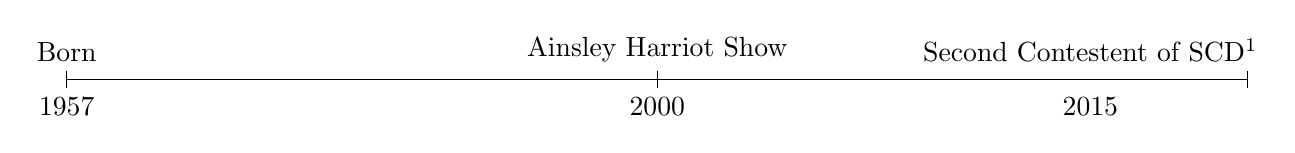
\begin{tikzpicture}[snake=zigzag, line before snake = 5mm, line after snake = 5mm]
   % draw horizontal line   
   \draw (0,0) -- (15,0);

   % draw vertical lines
   \foreach \x in {0,7.5,15}
     \draw (\x cm,3pt) -- (\x cm,-3pt);

   % draw nodes
   \draw (0,0) node[below=3pt] {$ 1957 $} node[above=3pt] { Born };
   \draw (7.5,0) node[below=3pt] {$ 2000 $} node[above=3pt] { Ainsley Harriot Show };
   \draw (13,0) node[below=3pt] {$ 2015 $} node[above=3pt] {Second Contestent of SCD\footnotemark};
 \end{tikzpicture}


\footnotetext{Strictly Come Dancing}

\subsection*{Education / Training}
\label{sec:orga1247ca}

``Harriott trained at Westminster Kingsway College (formerly Westminster Technical College), Harriott obtained an apprenticeship at Verrey's restaurant in the West End and later worked as a commis chef.''\cite{wikipedia}


\subsection*{What makes them famous?}
\label{sec:orga8f7d72}

"Harriett is famous from being the resident chef on 'Good Morning with Anne and Nick' and later the main presenter of 'Can't Cook, Won't Cook' and 'Ready Steady Cook', both shows involving members of the public."\cite{wikipedia}

He's also taken part in a documentary, specifically "Who Do You Think You Are?" 

Another large part of what makes him famous is the fact that he is a "best-selling author, publishing twelve books as well as numerous others in conjunction with his television shows."\cite{wikipedia} 

\newpage

Some other mentions are: 
\begin{itemize}
\item President of the TRIC\footnotemark from 2004-2005, and presented the awards for their ceremony that year
\item Played the Narrator in "The Rocky Horror Show" in three seperate theaters in 2010
\item Guest appearence in radio comedy show "Giles Wemmbley Hogg Goes Off" in 2008
\end{itemize}

\footnotetext{Television and Radio Industries Club}

\subsection*{Two of their signature recipes}
\label{sec:org56d279d}

\href{http://www.bbc.co.uk/food/recipes/\_81487}{Mustard and thyme crusted rib-eye of beef}\\
\href{http://www.bbc.co.uk/food/recipes/caribbeanjerkchicken\_86981}{Jerk chicken with rice, peas and fried plantain}

\subsubsection*{Why would you would (or would not) like to try the recipes}
\label{sec:org34da339}

I would love to try the Mustard and thyme crusted rib-eye, because I love beef, and there are a lot of good ingredients in the recipe like fresh thyme, chives and horseradish.

I would be a little more reluctant trying to Jerk chicken, because I'm not the biggest fan of kidney beans, or coconut milk. I could substitute the ingredients however, and the recipe is prepared in less than 30 minutes, and cooks in 10-30 minutes. 

\subsubsection*{List any unfamiliar items in each recipe and explain what they are}
\label{sec:org1cd5db5}

The nice thing about Ainsley's recipes is that they don't really involve and super complicated ingredients. The only ingredient I didn't know in the Jerk chicken recipe was Coriander, which ironically is one of the world's most commonly used herbs. The only ingredient I didn't know in the beef recipe was Dijon mustard, which is just a special mustard made with wine.

\newpage

\begin{thebibliography}{9}
\bibitem{wikipedia}
Wikipedia Contributors. "Ainsley Harriott." \textit{Wikipedia, The Free Encyclopedia.} Wikipedia, The Free Encyclopedia, 11 April. 2017. Web. 11 Jan. 2017.
\end{thebibliography}
\end{document}